\part{Algorithms}
\frame{\partpage}

\begin{frame}{What is an algorithm?}
	\pause\begin{center}
		A \textbf{sequence of instructions} which can be followed \textbf{step by step}
		to perform a \textbf{computational task}.
	\end{center}
\end{frame}

\begin{frame}{Programs vs algorithms}
	\begin{itemize}
		\pause\item A program is \textbf{specific} to a particular programming language and/or machine
		\pause\item An algorithm is \textbf{general}
		\pause\item An algorithm must be \textbf{implemented} as a program before a computer can run it
		\pause\item An algorithm generally performs \textbf{one task}, whereas a program may perform \textbf{many}
		\begin{itemize}
			\pause\item E.g.\ Microsoft Word is not an algorithm, but it implements many algorithms
			\pause\item E.g.\ it implements an algorithm for determining where to break a line of text,
				how much space to add to centre a line, etc.
		\end{itemize}
	\end{itemize}
\end{frame}

\begin{frame}{Algorithms outside computing}
	\begin{center}
		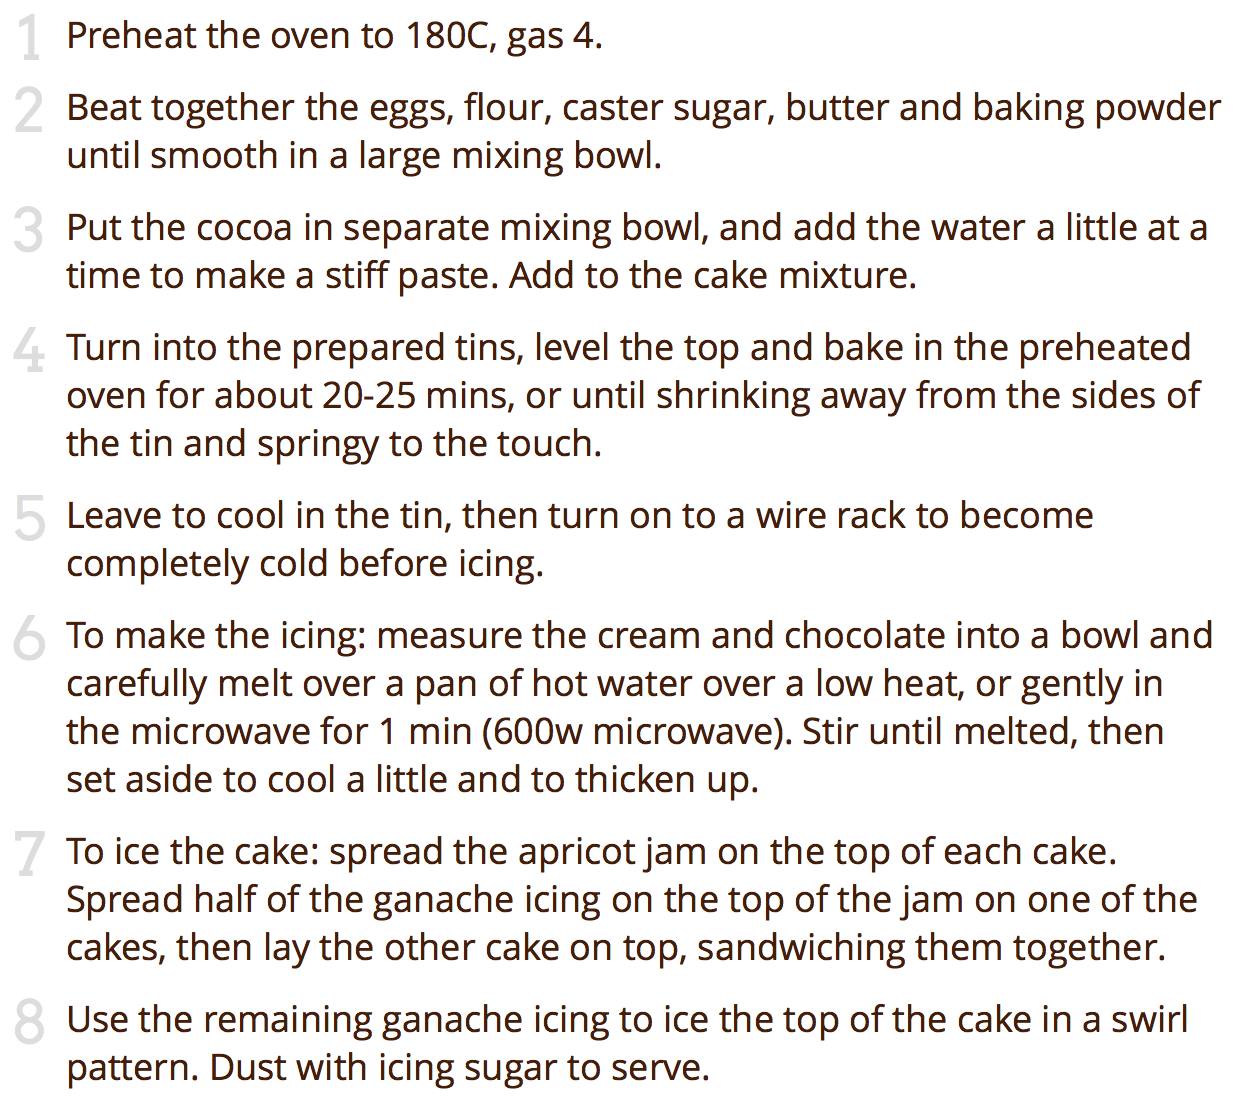
\includegraphics[height=0.8\textheight]{cake_recipe}
	\end{center}
\end{frame}

\begin{frame}{Algorithms outside computing}
	\begin{center}
		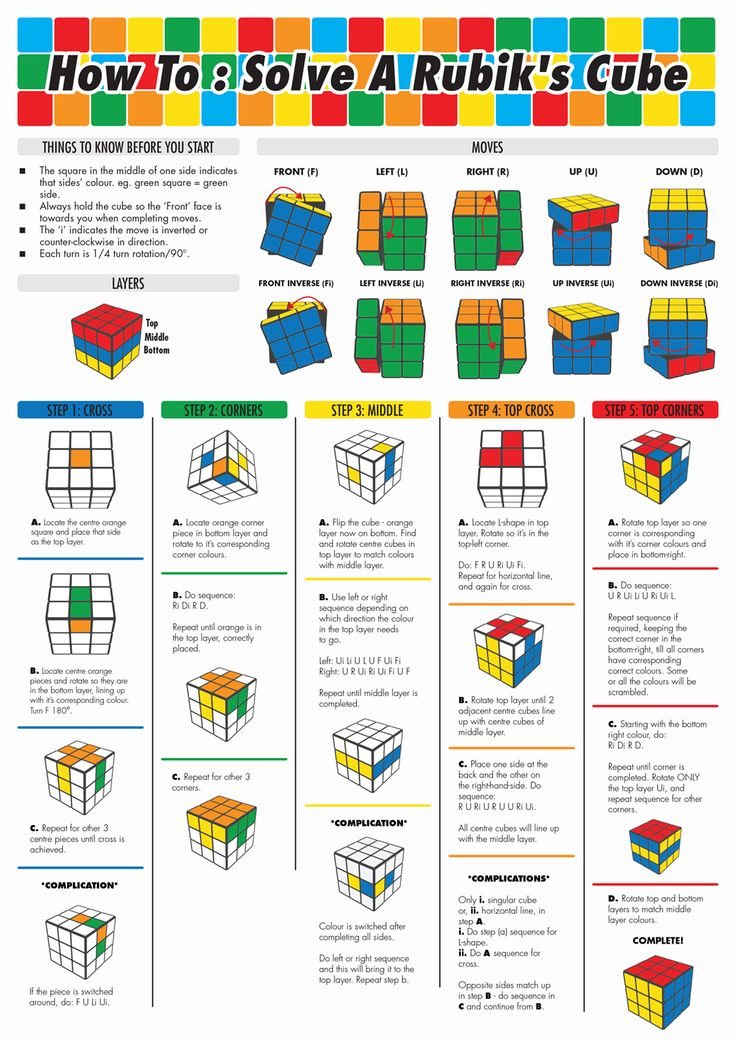
\includegraphics[height=0.8\textheight]{rubik_algorithm}
	\end{center}
\end{frame}
